\documentclass[letterpaper]{article}

\usepackage{natbib,alifeconf}  %% The order is important

\usepackage{hyperref}

\usepackage{subcaption}

\usepackage{hhline}

\usepackage{bm}

\ifdefined\mydraft
\mydraft
\fi

% *****************
%  Requirements:
% *****************
%
% - All pages sized consistently at 8.5 x 11 inches (US letter size).
% - PDF length <= 8 pages for full papers, <=2 pages for extended
%    abstracts.
% - Abstract length <= 250 words.
% - No visible crop marks.
% - Images at no greater than 300 dpi, scaled at 100%.
% - Embedded open type fonts only.
% - All layers flattened.
% - No attachments.
% - All desired links active in the files.

% Note that the PDF file must not exceed 5 MB if it is to be indexed
% by Google Scholar. Additional information about Google Scholar
% can be found here:
% http://www.google.com/intl/en/scholar/inclusion.html.


% If your system does not generate letter format documents by default,
% you can use the following workflow:
% latex example
% bibtex example
% latex example ; latex example
% dvips -o example.ps -t letterSize example.dvi
% ps2pdf example.ps example.pdf


% For pdflatex users:
% The alifeconf style file loads the "graphicx" package, and
% this may lead some users of pdflatex to experience problems.
% These can be fixed by editing the alifeconf.sty file to specify:
% \usepackage[pdftex]{graphicx}
%   instead of
% \usepackage{graphicx}.
% The PDF output generated by pdflatex should match the required
% specifications and obviously the dvips and ps2pdf steps become
% unnecessary.


% Note:  Some laser printers have a serious problem printing TeX
% output. The use of ps type I fonts should avoid this problem.


\title{Toward Open-Ended Fraternal Transitions in Individuality}
\author{Matthew Andres Moreno \and Charles Ofria \\
\mbox{}\\
BEACON Center, Michigan State University, East Lansing, MI 48824 \\
mmore500@msu.edu} % email of corresponding author

% For several authors from the same institution use the same number to
% refer to one address.
%
% If the names do not fit well on one line use
%         Author 1, Author 2 ... \\ {\Large\bf Author n} ...\\ ...
%
% If the title and author information do not fit in the area
% allocated, place \setlength\titlebox{<new height>} after the
% \documentclass line where <new height> is 2.25in



\begin{document}
\maketitle

\begin{abstract}
% Abstract length should not exceed 250 words

Evolutionary transitions of individuality have been key to the complexification and diversification of biological life.
Realizing and studying such transitions are thought to be a key factor with respect to the question of open-ended evolution.
In order to study evolutionary transitions of individuality, we must devise a system in which we expect such transitions to occur in a detectable manner.
To this end, we introduce the DISHTINY (DIStributed Hierarchical Transitions of IndividualitY) platform, which seeks to achieve this goal by explicitly registering organisms in cooperating groups that coordinate spatiotemporally to maximize the harvest of a resource.
We lay out the design of DISHTINY and discuss its scalability.
Then, we use ecological competition and evolutionary experiments to demonstrate selection for and emergence of high-level individuality using simple organisms that evolve parameters for manually-designed strategies.
In evolutionary experiments, we observe reproductive division of labor and close cooperation between individuals registered to the same cooperating group, including resource-sharing and emergence of an apoptosis response to somatic mutation.
Ecological competition experiments demonstrate that genotypes that encode higher-level individuality outcompete those that encode lower-level individuality.

\end{abstract}


\section{Introduction}

Artificial Life researchers design systems that exhibit properties of biological life in order to better understand their dynamics and, often, to apply these principles toward engineering applications such as artificial intelligence \citep{bedau2003artificial}.
Studies of evolution have been of particular interest to the community, especially in regard to how organisms are produced with increasing sophistication and complexity \citep{goldsby2017increasing}.
This particular issue is often described as ``open-ended evolution.''
Although precise definitions and measures of open-ended evolution are still being established, this term is generally understood to refer to evolving systems that exhibit the continued production of novelty \citep{taylor2016open}.
Evolutionary transitions in individuality, which are key to the complexification and diversification of biological life \citep{smith1997major}, have been highlighted as key research targets with respect to the question of open-ended evolution \citep{ray1996evolving, banzhaf2016defining}.
In an evolutionary transition of individuality, a new, more complex replicating entity is derived from the combination of cooperating replicating entities that have irrevocably entwined their long-term fates \citep{west2015major}.
Eusocial insect colonies and multicellular organisms exemplify this phenomenon \citep{smith1997major}.
Like the definition of open-ended evolution, the notion of what constitutes an evolving individual is not concretely established.
Commonly indicated features include:
close coordination and cooperation, reproductive division of labor, reproductive bottlenecks, and loss of ability to replicate independently
\citep{ereshefsky2015rethinking, bouchard2013symbiotic}.
% @CAO: I wasn't sure how reproductive lineages could be see to shift without first recognizing the transition...
%reproductive lineages (e.g., parent-offspring relationships) at the level of the ensemble

Major challenges in studying evolutionary transitions in individuality include (1) determining the environmental conditions that will promote such a transition and then (2) recognizing that a transition has occurred.
In order to begin exploring transitions in individuality, we must devise a system in which we expect such transitions to occur repeatably and in a detectable manner.
Once we can consistently induce and observe evolutionary transitions in individuality, we may subsequently proceed to relax aspects of such a system to explore in greater detail what conditions are necessary to induce transitions and how transitions can be detected.
For now, we will focus on these initial goals in the context of fraternal transitions in individuality --- events where closely-related kin come together or stay together to form a higher-level organism.

To this end, we introduce the DISHTINY (DIStributed Hierarchical Transitions in IndividualitY) platform, which seeks to achieve the evolution of transitions in individuality by explicitly registering organisms in cooperating groups that coordinate spatiotemporally to maximize the harvest of a resource.
Detection of such a transition in DISHTINY is accomplished by identifying resource-sharing and reproductive division of labor among organisms registered to the same cooperating group.
We designed this system such that hierarchal transitions across an arbitrary number of levels of individuality can be selected for and meaningfully detected.
We have focused this system on a rigid form of major transition using simple organisms, but the underlying principles can be applied to a wide range of artificial life systems.
Furthermore, DISHTINY is decentralized and amenable to massive parallelization via distributed computing.
We believe that such scalability --- with respect to both concept and implementation --- is an essential consideration in the pursuit of artificial systems capable of generating complexity and novelty rivaling that of biological life via open-ended evolution \citep{ackley2011pursue, ackley2016indefinite}.


\section{Methods}

We manually designed strategies that organisms could use to cooperate to experimentally demonstrate that the dishtiny framework selects for detectable hierarchical transitions of individuality.

\subsection{dishtiny}
We will begin by discussing at a single hierarchicical level, then lay out how the system scales to multiple levels

* resource distribution

* signaling

This means that at each level organisms benefit from cooperating with a medium-sized, diamond-shaped group : it has to be ``just right'' too small and they'll miss out on resource that passes over; too big and they'll activate erroneously and quickly bankrupt themselves.
They are forced to control the size and shape of this cooperating through their reproductive choices --- offspring .

Interestingly, signaling can lead to a standing wave and kill u

* hierarchy

\subsection{test organisms}

each organism consisted of a set of floating-point values that described

* res_pool

* avoid_over

* off_ch_cap

* sort_off

* damage_suicide

We would expect a zero-level individual to exhibit a genotype along the lines of

describe

We would expect a first-level individual to exhibit a genotype along the lines of

describe

Finally, we would expect a second-level individual to exhibit a genotype along the lines of

describe

\subsection{implementation}

code is available here \url{https://github.com/mmore500/dishtiny}

data and visualizations are available here \url{https://osf.io/ewvg8/}


\section{Results and Discussion}

\begin{figure*}%[!htbp]

\begin{center}
\setlength\tabcolsep{1.5pt} % default value: 6pt
\begin{tabular}{ | c || c c c | c c c | c | c | }
  \multicolumn{8}{c}{} & \multicolumn{1}{c}{Control} \\
  \multicolumn{1}{c}{} & \multicolumn{3}{c}{Competitors} & \multicolumn{3}{c}{Mean Dominant ($\pm S.D.$)} & \multicolumn{1}{c}{ Pop Mean ($\pm S.D.$)} & \multicolumn{1}{c}{ Pop Mean ($\pm S.D.$)} \\
 \cline{2-9}
  \multicolumn{1}{c|}{} & \tiny{$P_{1} = 1.0$} & \tiny{$P_{2} = P_{1}$} & \tiny{$P_{2} > P_{1}$} & \tiny{$P_{1} = 1.0$} & \tiny{$1.0 > P_{1} > P_{2}$} & \tiny{$P_{2} \geq P_{1}$} & \tiny{\textit{all}} & \tiny{\textit{all}}  \\
 \hline
 $Upd.$ & 25M & 25M & 25M & 25M & 25M & 25M & 200k & 200k \\
 $n$ & 1 & 1 & 1 & 9 & 7 & 34 & 50 & 50 \\
 \hhline{|=||===|===|=|=|}
 $A_1$ & 0.00 & 0.00 & 0.89 & $0.23 \pm 0.35$ & $0.50 \pm 0.47$ & $0.57 \pm 0.46$ & $0.51 \pm 0.14$ & $0.46 \pm 0.30$\\
 $A_2$ & 1.00 & 1.00 & 1.00 & $1.00 \pm  0.00$ & $1.00 \pm 0.00$ & $1.00 \pm 0.00$ & $1.00 \pm 0.00$ & $1.00 \pm 0.00$ \\
 \hline
 $P_{c}$ & 0.00 & 0.00 & 0.00 & $0.00 \pm 0.00$ & $0.00 \pm 0.00$ & $0.03 \pm 0.05$ & $0.07 \pm 0.03$ & $0.00 \pm 0.00$ \\
 $P_1$ & 1.00 & 0.50 & 0.00 & $1.00 \pm 0.00$ & $0.60 \pm 0.07$ & $0.28 \pm 0.16$ & $0.39 \pm 0.11$ & $0.04 \pm 0.08$ \\
 $P_2$ & 0.00 & 0.50 & 1.00 & $0.00 \pm 0.00$ & $0.40 \pm 007$ & $0.69 \pm 0.14$ & $0.54 \pm 0.11$ & $0.96 \pm 0.08$ \\
 \hline
 $C_1$ & 3.13 & 3.45 & 2.04 & $3.90 \pm 0.60$ & $3.38 \pm 0.33$ & $3.03 \pm 0.69$ & $3.38 \pm 0.23$ & $8.21 \pm 5.45$ \\
 $C_2$ & 233.2 & 238.6 & 290.2 & $230.6 \pm 71.1$ & $192.7 \pm 45.3$ & $271.6 \pm 73.6 $ & 99$.2 \pm 7.4 $& 350$.0 \pm 92.1 $ \\
 \hline
 $E_{c}$ & 0.87 & 0.14 & 4.20 & $0.29 \pm 0.37$ & $0.44 \pm 0.59$ & $0.21 \pm 0.75$ & $1.43 \pm 0.38$ & $2.77 \pm 1.50$ \\
 $E_1$ & 33.4 & 11.7 & 4.80 & $47.2 \pm 21.7$ & $21.3 \pm 12.0$ & $4.62 \pm 7.05$ & $31.5 \pm 6.6$ & $6.72 \pm 9.58$ \\
 $E_2$ & 341.4 & 397.4 & 321.1 & $231.2 \pm 94.3$ & $283.1 \pm 57.0$ & $325.4 \pm 68.9$ & $240.0 \pm 30.0$ & $317.5 \pm 55.2$ \\
 \hline
 $M_{c}$ & 0.11 & 1.00 & 0.66 & $0.33 \pm 0.41$ & $0.74 \pm 0.31$ & $0.67 \pm 0.35$ & $0.50 \pm 0.11$ & $0.20 \pm 0.23$ \\
 $M_1$ & 0.00 & 1.00 & 0.40 & $0.52 \pm 0.41$ & $0.65 \pm 0.46$ & $0.68 \pm 0.38$ & $0.50 \pm 0.12$ & $0.50 \pm 0.34$ \\
 $M_2$ & 0.00 & 0.44 & 1.00 & $0.45 \pm 0.39$ & $0.52 \pm 0.37$ & $0.50 \pm 0.42$ & $0.50 \pm 0.13$ & $0.50 \pm 0.33$ \\
 \hline
 $S_1$ & 0.00 & 1.00 & 1.00 & $0.65 \pm 0.38$ & $0.55 \pm 0.40$ & $0.47 \pm 0.42$ & $0.48 \pm 0.11$ & $0.48 \pm 0.34$ \\
 $S_2$ & 0.00 & 0.01 & 0.46 & $0.51 \pm 0.43$ & $0.35 \pm 0.39$ & $0.45 \pm 0.39$ & $0.49 \pm 0.13$ & $0.44 \pm 0.31$ \\
 \hline
\end{tabular}
\end{center}
\caption{
Enumerations for genotypes used as seeds for competition experiments (left) and enumerations for mean values of the most abundant genotype at the end of evolutionary runs (right), both sorted by resource-caching strategy.
}
\label{fig:genotypes}
\end{figure*}


\begin{figure*}%[!htbp]
\begin{center}
\thinmuskip=-2mu
\thickmuskip=-2mu
\nulldelimiterspace=-1pt
\scriptspace=0pt
\begin{subfigure}[b]{0.66\columnwidth}
  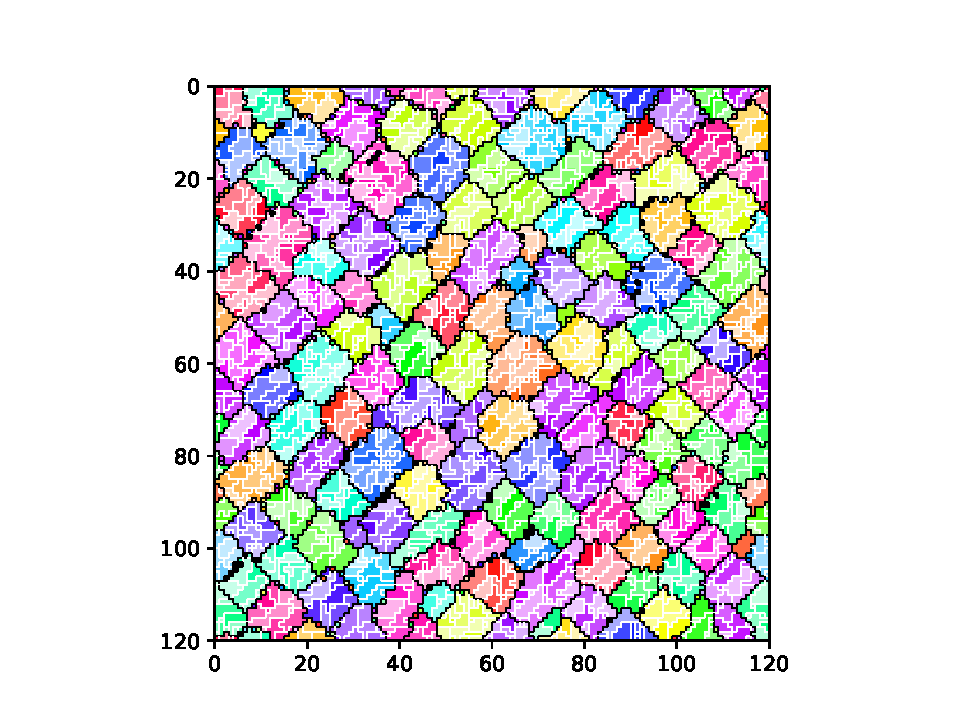
\includegraphics[width=\columnwidth,trim={2.5cm 0.5cm 2.5cm 1cm},clip]{img/ChannelMap_1022_update19500000}
  \caption{Mean $P_{c} = 0.77$, $P_1 = 0.09$, $P_2 = 0.14$; gen. 20,475}
  \label{fig:ChannelMap_1022}
\end{subfigure}%
\begin{subfigure}[b]{0.66\columnwidth}
  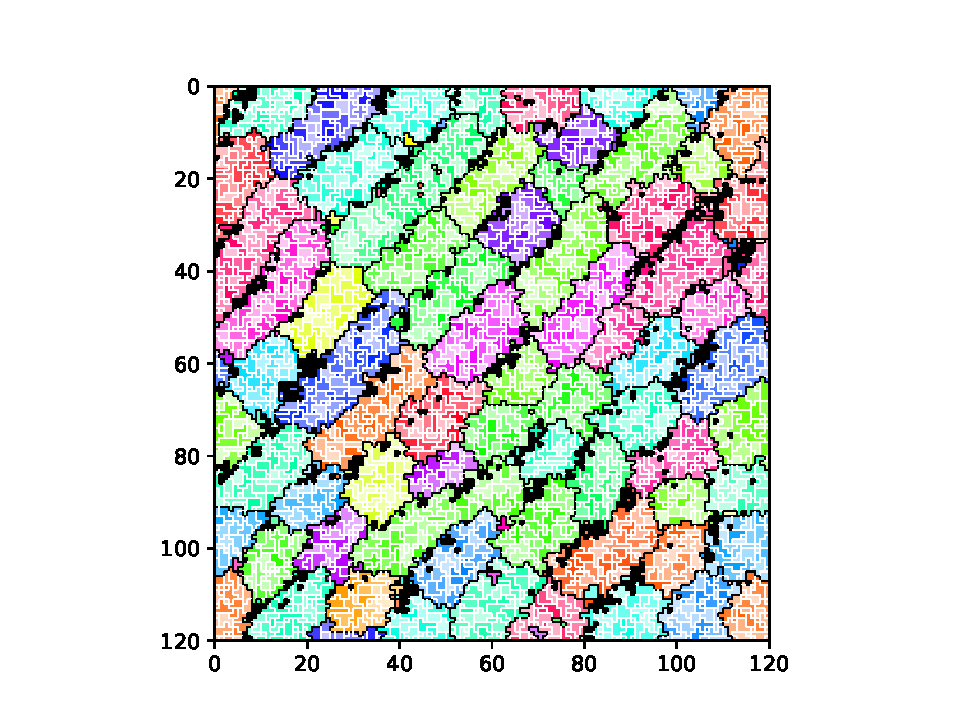
\includegraphics[width=\columnwidth,trim={2.5cm 0.5cm 2.5cm 1cm},clip]{img/ChannelMap_1041_update19500000}
  \caption{Mean $P_1 = 1.0$; gen. 23,971\\~}
  \label{fig:ChannelMap_1041}
\end{subfigure}%
\begin{subfigure}[b]{0.66\columnwidth}
  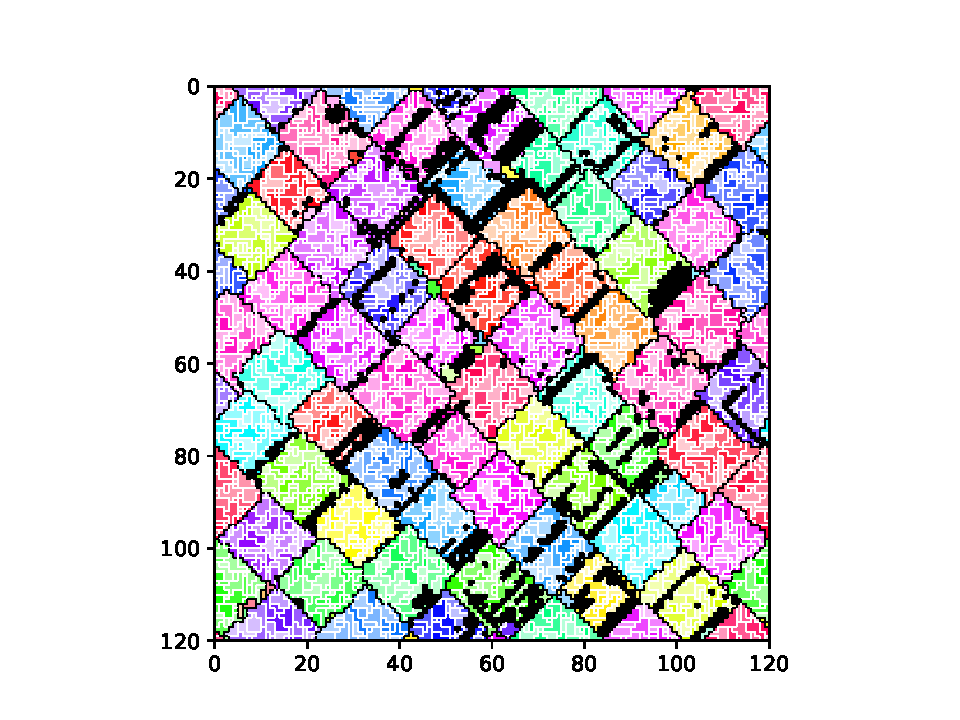
\includegraphics[width=\columnwidth,trim={2.5cm 0.5cm 2.5cm 1cm},clip]{img/ChannelMap_1008_update19500000}
  \caption{Mean $P_2 = 1.0$; gen. 25,841\\~}
  \label{fig:ChannelMap_1008}
\end{subfigure}

\caption{
End state of same-channel signaling networks in replicates where cell- (\ref{fig:ChannelMap_1022}), first- (\ref{fig:ChannelMap_1041}), and second-level (\ref{fig:ChannelMap_1008}) individuality dominated.
(Cell-level individuals are single cells that retain collected resource exclusively for their own use, first-level individuals are level-one same-channel multi-cellular networks that primarily assign collected resource for collective use among level-one channel mates, and second-level individuals are level-two same-channel multi-cellular networks that primarily assign collected resource for collective use among level-two channel mates.)
Level-one channels are coded by color saturation and level-two channels are coded by color hue.
A single cell-like organism occupies each grid tile except for black tiles, which are empty.
}
\label{fig:outcome_grids}
\end{center}
\end{figure*}


\begin{figure*}%[!htbp]
\begin{center}

\begin{subfigure}[b]{0.33\columnwidth}
  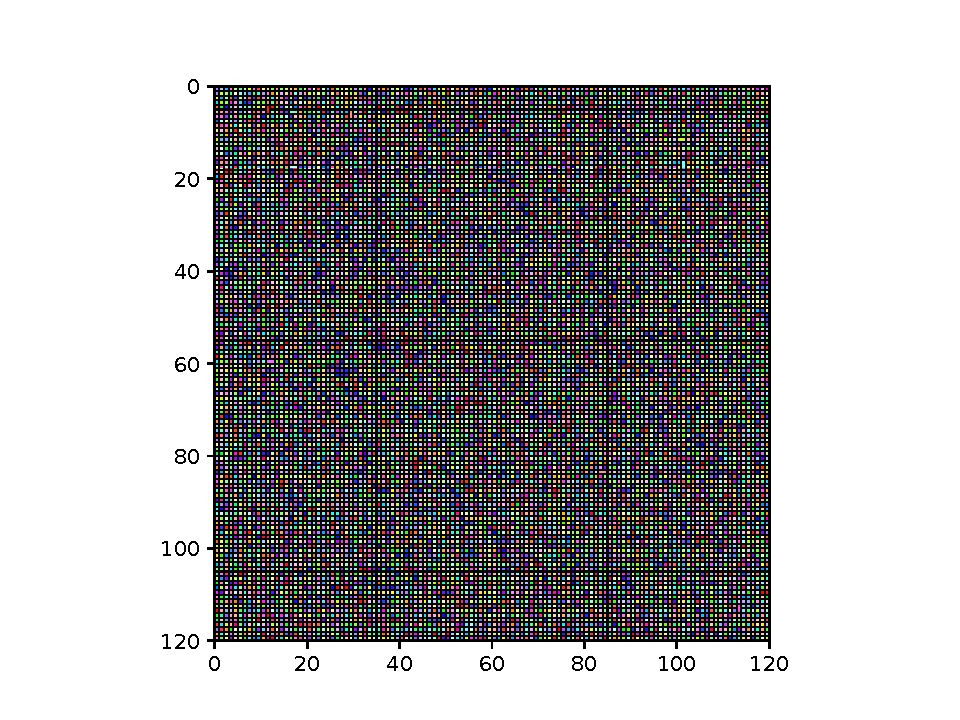
\includegraphics[width=\columnwidth,trim={2.5cm 0.5cm 2.5cm 1cm},clip]{img/ChannelMap_1007_update0}
  \vspace{-5ex}
  \caption{Update 0; cell gen. 0}
  \label{fig:ChannelMap_1007_update0}
\end{subfigure}%
\begin{subfigure}[b]{0.33\columnwidth}
  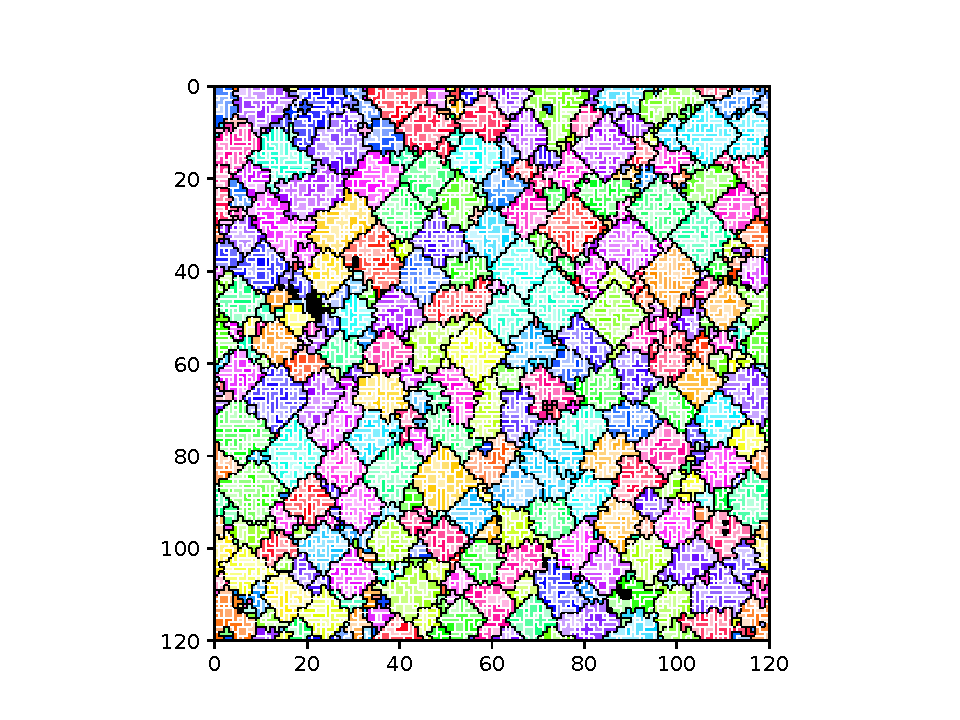
\includegraphics[width=\columnwidth,trim={2.5cm 0.5cm 2.5cm 1cm},clip]{img/ChannelMap_1007_update55520}
  \vspace{-5ex}
  \caption{Update 55520; cell gen. 103}
  \label{fig:ChannelMap_1007_update55520}
\end{subfigure}%
\begin{subfigure}[b]{0.33\columnwidth}
  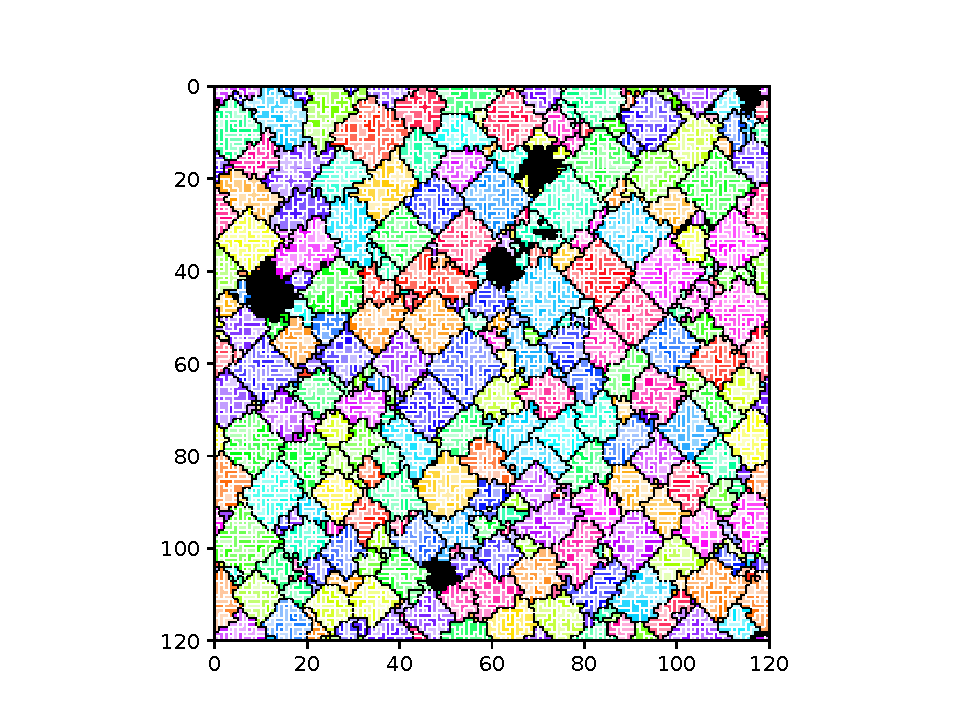
\includegraphics[width=\columnwidth,trim={2.5cm 0.5cm 2.5cm 1cm},clip]{img/ChannelMap_1007_update277600}
  \vspace{-5ex}
  \caption{Update 277600; cell gen. 563}
  \label{fig:ChannelMap_1007_update277600}
\end{subfigure}

\begin{subfigure}[b]{0.33\columnwidth}
  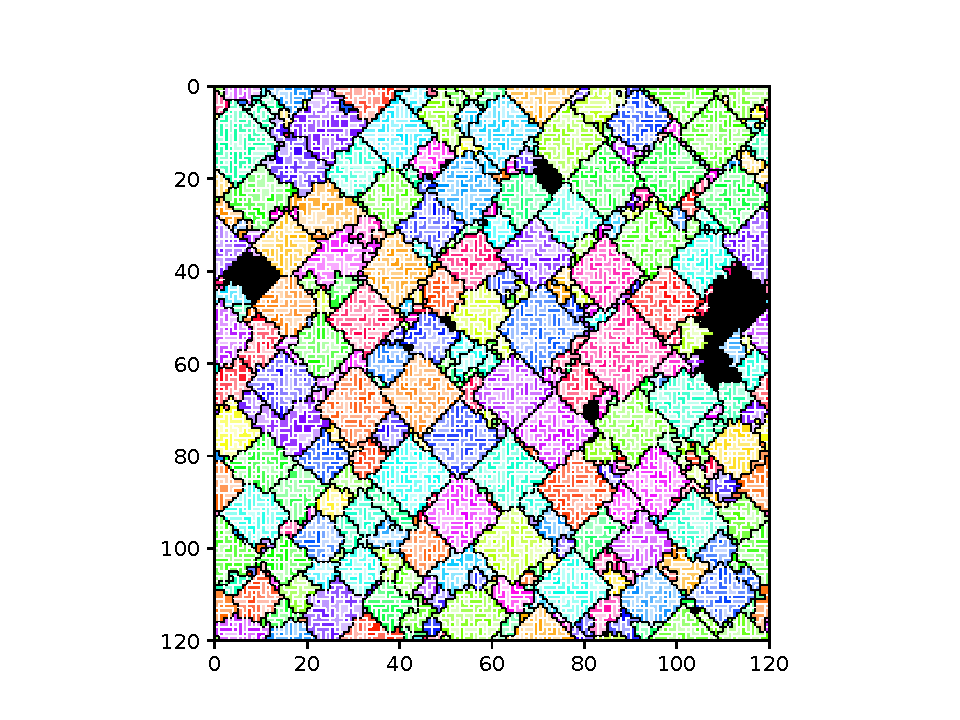
\includegraphics[width=\columnwidth,trim={2.5cm 0.5cm 2.5cm 1cm},clip]{img/ChannelMap_1007_update500000}
  \vspace{-5ex}
  \caption{Update 500000; cell gen. 1072}
  \label{fig:ChannelMap_1007_update500000}
\end{subfigure}%
\begin{subfigure}[b]{0.33\columnwidth}
  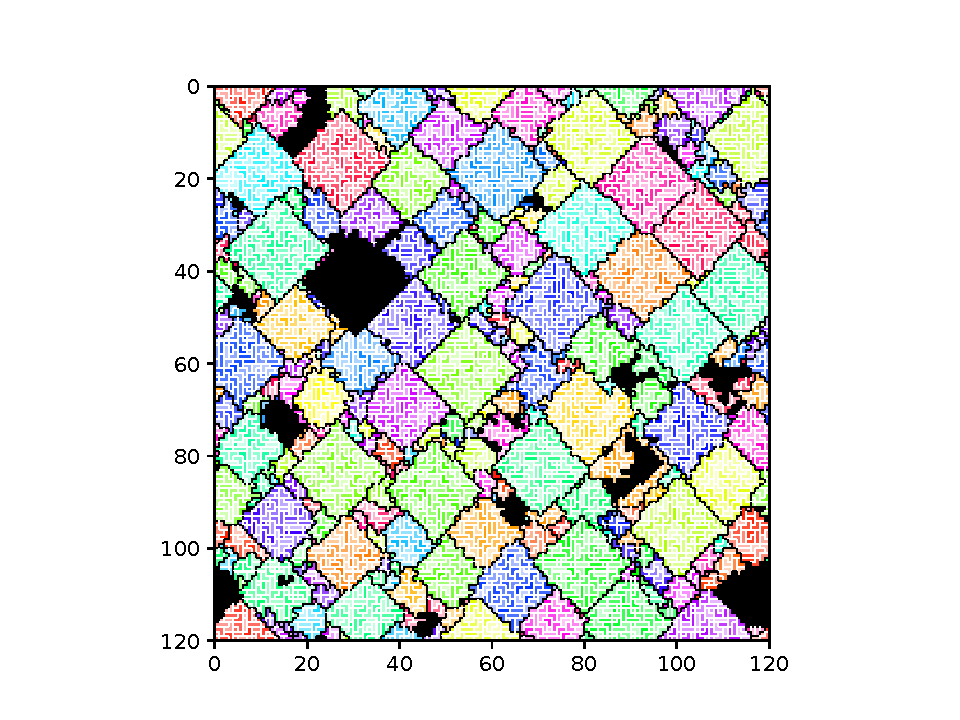
\includegraphics[width=\columnwidth,trim={2.5cm 0.5cm 2.5cm 1cm},clip]{img/ChannelMap_1007_update1000000}
  \vspace{-5ex}
  \caption{Update 1000000; cell gen. 2405}
  \label{fig:ChannelMap_1007_update1000000}
\end{subfigure}%
\begin{subfigure}[b]{0.33\columnwidth}
  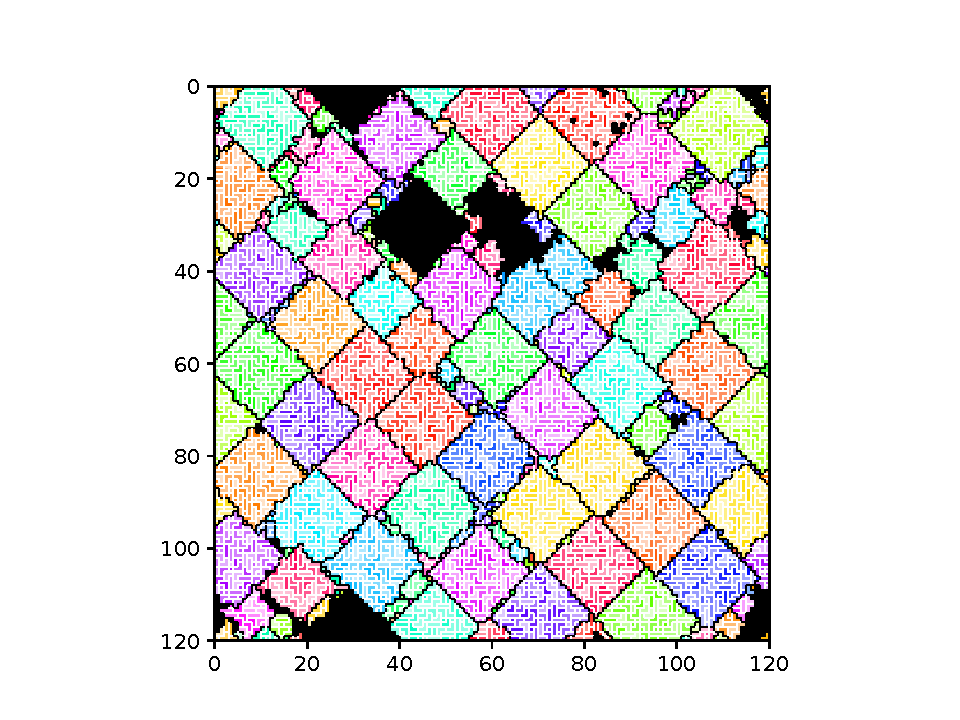
\includegraphics[width=\columnwidth,trim={2.5cm 0.5cm 2.5cm 1cm},clip]{img/ChannelMap_1007_update2000000}
  \vspace{-5ex}
  \caption{Update 2000000; cell gen. 4974}
  \label{fig:ChannelMap_1007_update2000000}
\end{subfigure}

\caption{
Progression of same-channel level-one and level-two signaling networks states in an evolutionary run where level-two resource sharing evolved.
Level-one channels are coded by color saturation and level-two channels are coded by color hue.
A single cell-like organism occupies each grid tile except for black tiles, which are empty.
Level-one same-channel groups appear as uniformly-colored clumps, bounded by a white border.
Level-two same-channel groups appear as same-hue amalgamations of level-one groups, bounded by a black border.
}
\label{fig:grid_progression}
\end{center}
\end{figure*}


\begin{figure*}%[!htbp]
\begin{center}


\begin{subfigure}[b]{0.9\columnwidth}
  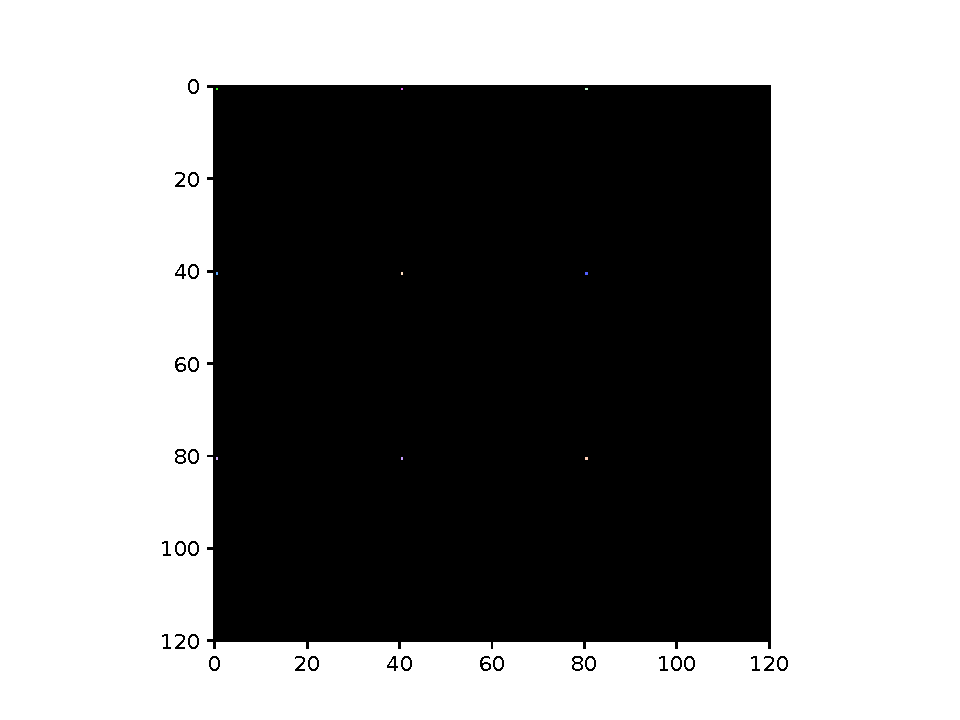
\includegraphics[width=\columnwidth,trim={2.5cm 0.5cm 2.5cm 1cm},clip]{img/ChannelMap_1030_update0}
  \caption{Update 0; cell gen. 0}
  \label{fig:ChannelMap_1030_update0}
\end{subfigure}%
\begin{subfigure}[b]{0.9\columnwidth}
  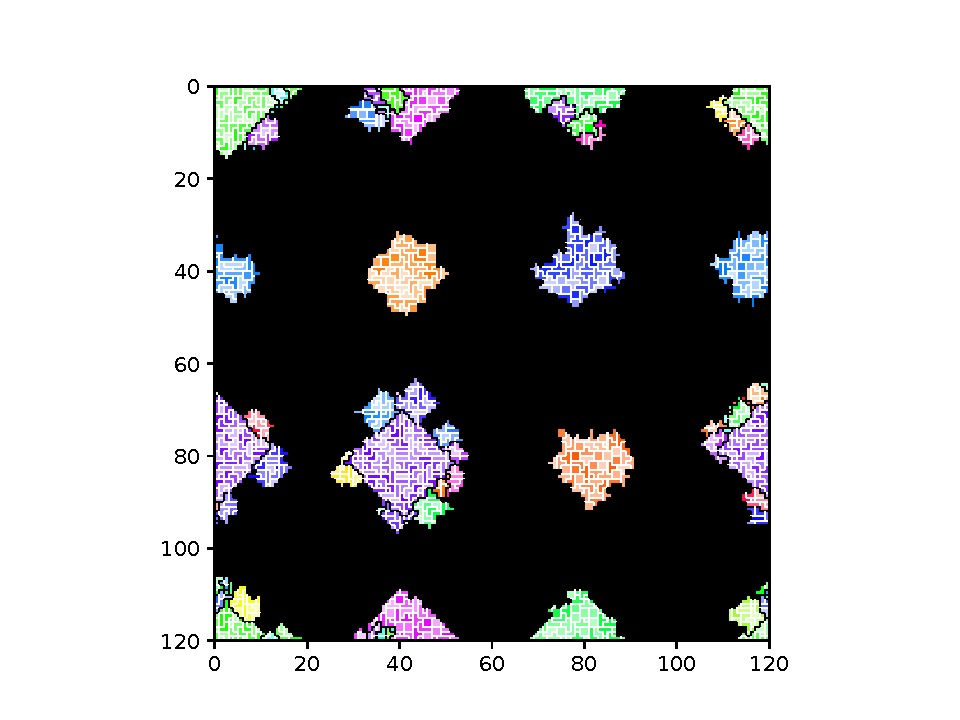
\includegraphics[width=\columnwidth,trim={2.5cm 0.5cm 2.5cm 1cm},clip]{img/ChannelMap_1030_update5552}
  \caption{Update 5552; cell gen. 4}
  \label{fig:ChannelMap_1030_update55520}
\end{subfigure}

\begin{subfigure}[b]{0.9\columnwidth}
  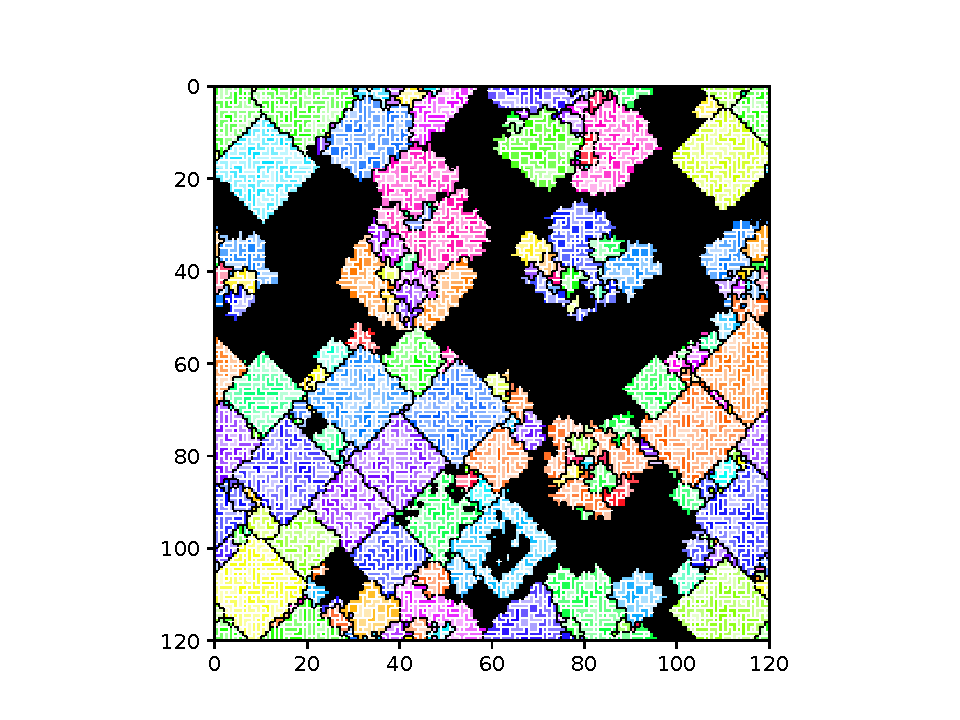
\includegraphics[width=\columnwidth,trim={2.5cm 0.5cm 2.5cm 1cm},clip]{img/ChannelMap_1030_update11104}
  \caption{Update 1104; cell gen. 9}
  \label{fig:ChannelMap_1030_update277600}
\end{subfigure}%
\begin{subfigure}[b]{0.9\columnwidth}
  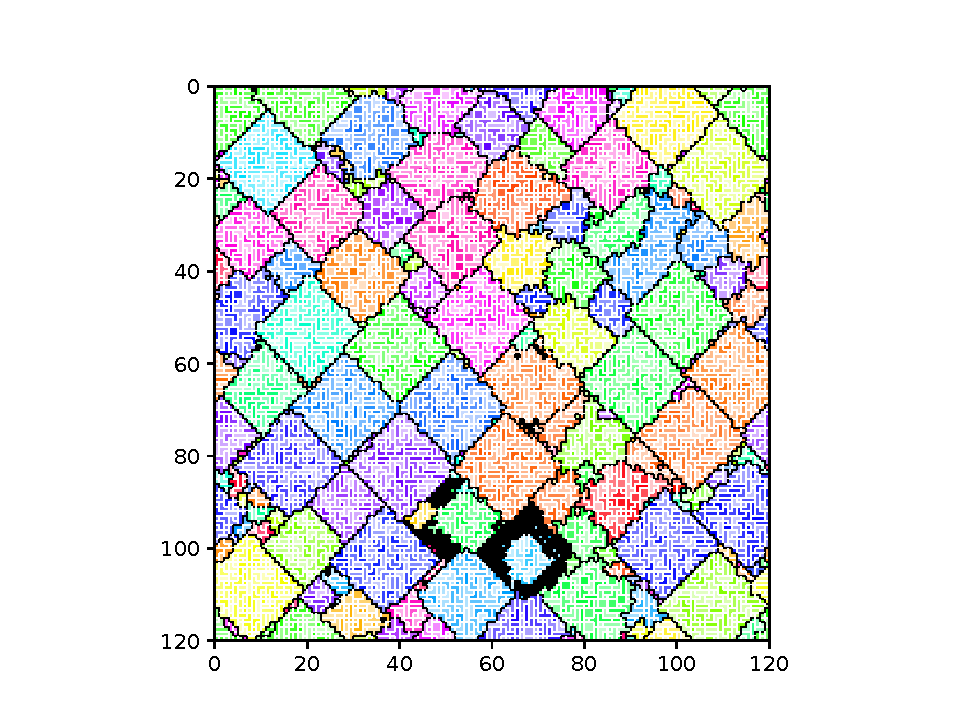
\includegraphics[width=\columnwidth,trim={2.5cm 0.5cm 2.5cm 1cm},clip]{img/ChannelMap_1030_update22208}
  \caption{Update 22208; cell gen. 32}
  \label{fig:ChannelMap_1030_update22208}
\end{subfigure}

\begin{subfigure}[b]{0.9\columnwidth}
  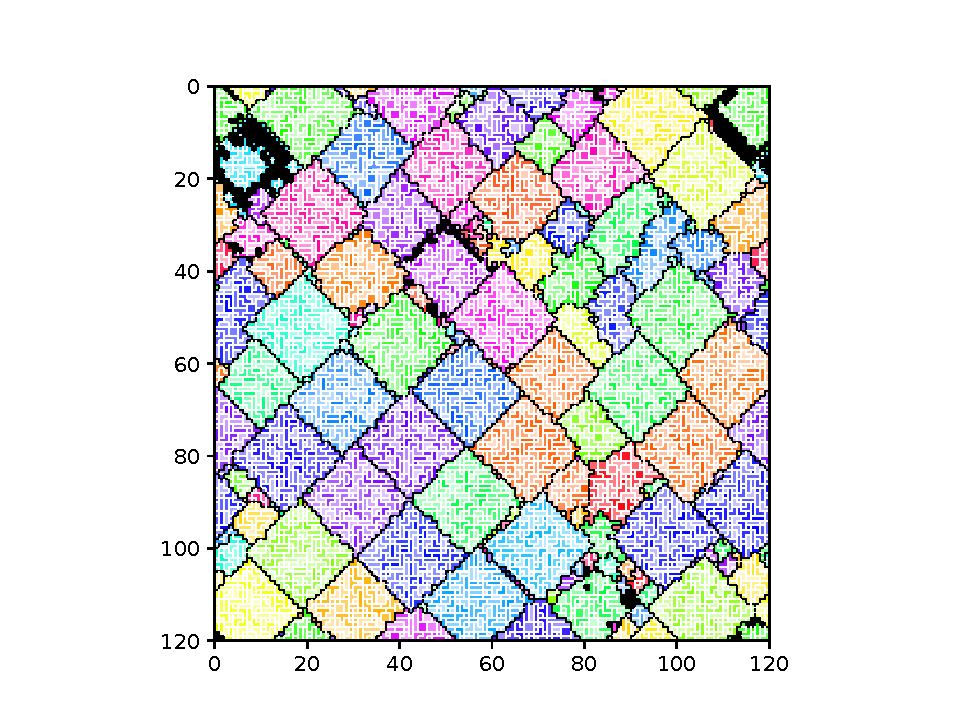
\includegraphics[width=\columnwidth,trim={2.5cm 0.5cm 2.5cm 1cm},clip]{img/ChannelMap_1030_update55520}
  \caption{Update 55520; cell gen. 107}
  \label{fig:ChannelMap_1030_update1000000}
\end{subfigure}%
\begin{subfigure}[b]{0.9\columnwidth}
  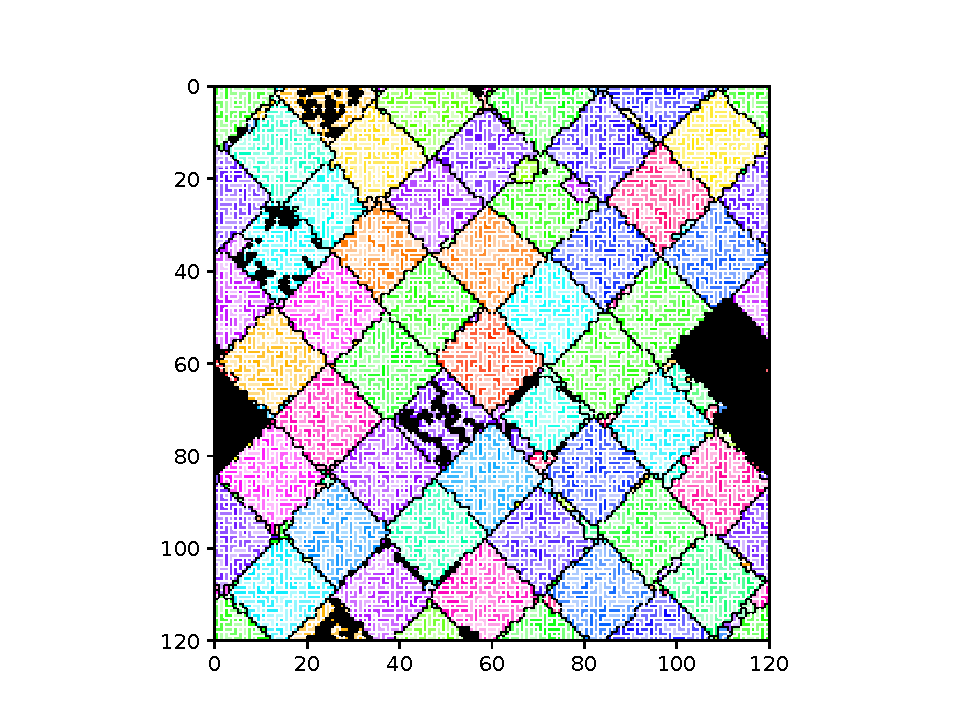
\includegraphics[width=\columnwidth,trim={2.5cm 0.5cm 2.5cm 1cm},clip]{img/ChannelMap_1030_update1500000}
  \caption{Update 1500000; cell gen. 3511}
  \label{fig:ChannelMap_1030_update1500000}
\end{subfigure}
\caption{
Progression of of same-channel level-one and level-two signaling networks states in a competition run.
We seeded the grid with three copies of each of three champion genotypes from evolutionary trials.
Then, with mutation disabled to prevent further evolution, the genotypes competed.
Level-one channels are coded by color saturation and level-two channels are coded by color hue.
A single cell-like organism occupies each grid tile except for black tiles, which are empty.
}
\label{fig:eco_progression}
\end{center}
\end{figure*}


\begin{figure}%[!htbp]
\begin{center}
\thinmuskip=-2mu
\thickmuskip=-2mu
\nulldelimiterspace=-1pt
\scriptspace=0pt

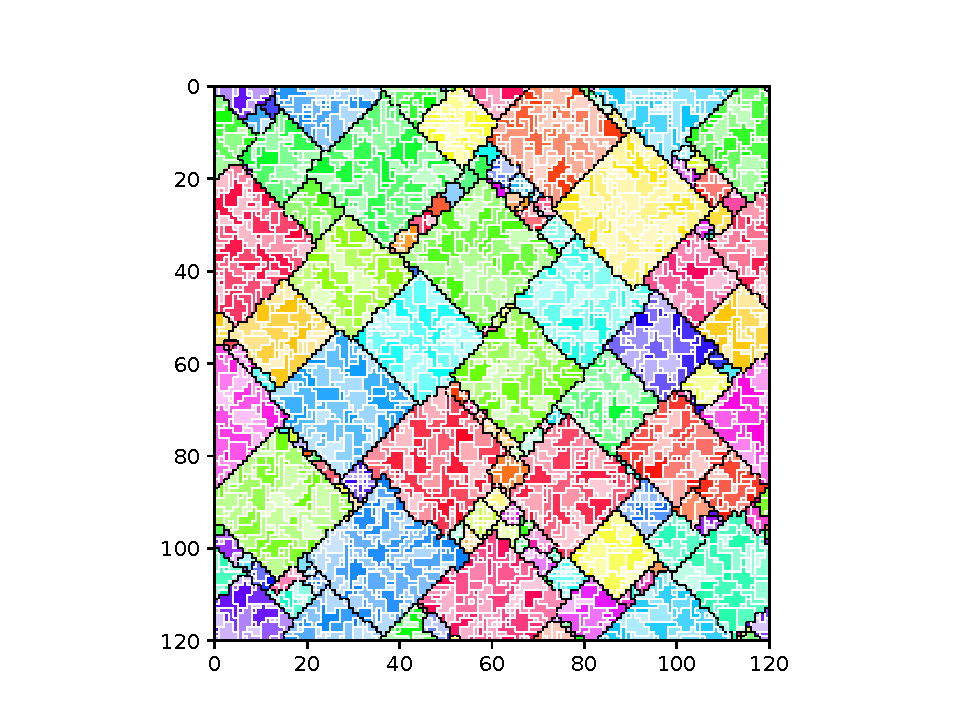
\includegraphics[width=\columnwidth,trim={2.5cm 0.5cm 2.5cm 1cm},clip]{img/ChannelMap_1018_update249840}

\caption{
End state of same-channel signaling networks in a randomly chosen replicate from the control treatment.
Update 249840, cell generation 5384.
Level-one channels are coded by color saturation and level-two channels are coded by color hue.
A single cell-like organism occupies each grid tile except for black tiles, which are empty.
}
\label{fig:outcome_control}
\end{center}
\end{figure}


Cell-, first-, and second-level individuals were all observed at the conclusion of different runs of our evolutionary simulation (mean generation 37,168; $s=4,684$).
The criteria used to discern these outcomes are described below.
Figure \ref{fig:outcome_grids} shows the level-one and level-two signaling networks at the end of runs where cell-, first-, and second-level individuality evolved, respectively.
Figure \ref{fig:grid_progression} shows a time series of signaling network snapshots in an evolutionary run where first-level individuality evolved.
Cell-level individuals appear to form with comparatively large level-one signaling networks that are arranged into amorphous level-two signaling networks.
Zeroth-level individuals appear to form elongated cigar-shaped level-two amalgamations of diverse level-one networks.
First-level individuals appear to form highly regular diamond-shaped level-two amalgamations of diverse level-one networks.

Figure \ref{fig:genotypes} describes predominant genotypes observed at the end of our evolutionary simulations.
With a single exception, nearly all evolved genotypes had $A_2$ fixed at or very near $1.0$ (i.e., population mean $A_2 \geq 0.993$).
So, reproduction over cells sharing the same level-two channel was near-universally avoided;
genotypes evolved so that cells declined to reproduce when they were located at the interior of level-two same-channel signaling networks.

However, a variety of resource-caching strategies evolved.
Most-abundant genotypes at the end of evolutionary runs included strategies where resource was primarily cached in an organism's individual stockpile (i.e., $P_{c} > P_1, P_2$), strategies where resource was primarily cached in an organism's level-one signaling network's pool (i.e., $P_1 > P_{c}, P_2$), and strategies where resource was primarily cached in an organism's level-two signaling network's pool (i.e., $P_2 > P_{c}, P_1$).
Among 33 trials, selfish cell-level hoarders dominated at the end of two replicates, level-one resource-sharing dominated in 16 replicates, and level-two resource sharing dominated in 15 replicates.

Given the near-ubiquitous nature of cooperation with regard to reproductive division of labor at the level-two same-channel signaling network, it was on this basis of resource caching strategy that we drew distinctions between cell-, first-, and second-level individuality.
(The single predominant genotype with $A_2 = 0.91$ had $P_1 = 1.0$, so was not sharing resource on the level-two same-channel resource pool).

Next, we wanted to compare cell-, first-, and second-level individuals to determine which genotype was the most fit in the DISHTINY platform environment.
We ran competition experiments between the the dominant genotypes from the run with greatest mean $P_{c}$, the run with greatest mean $P_1$, and the run with greatest mean $P_2$.
In 22 out of 191 trials performed fixation was reached by update 1.5 million.  The cell-level individuality genotype dominated in one trial, the first-level individuality genotype dominated in 12 trials, and the first-level individuality genotype dominated in 178 trials.
These results show that in the absence of mutation, first-level individuals tend to exhibit greater fitness than first- and cell-level individuals ($p < 0.0001$; RR 2.8; two-tailed exact test).

\begin{figure}[t]
\begin{center}

\begin{subfigure}[b]{\columnwidth}
  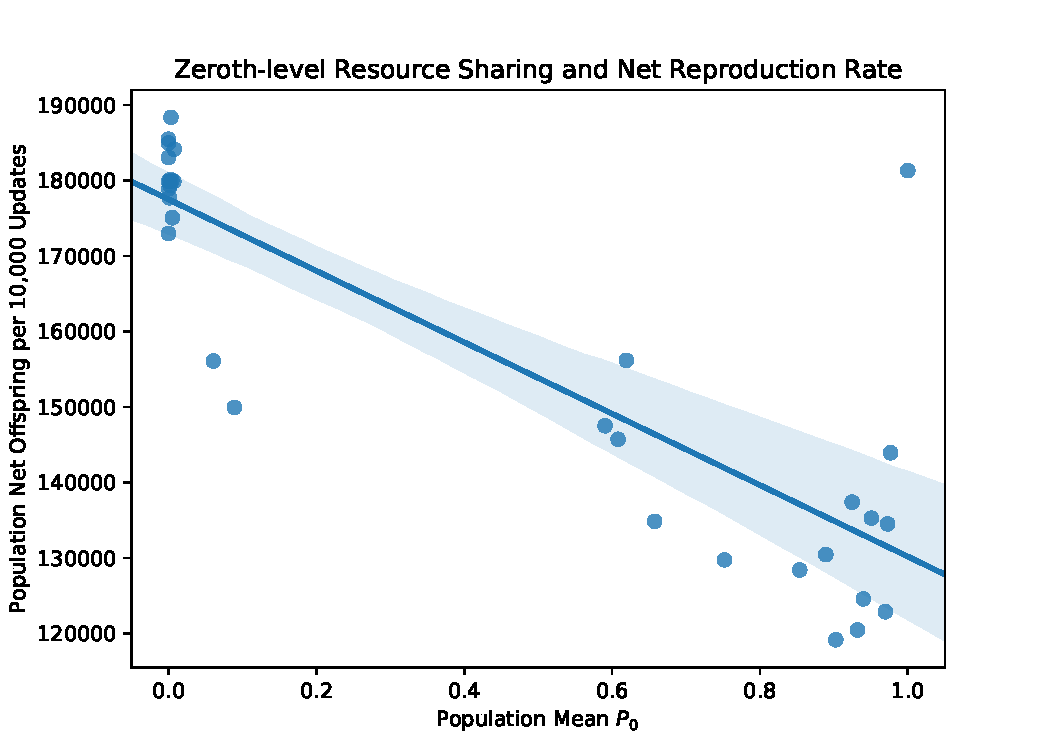
\includegraphics[width=\columnwidth]{img/mean_res_pool1_vs_net_reproduction}
  \caption{
  Correlation plot of population mean $P_1$ and population net reproduction rate.
  }
  \label{fig:mean_res_pool1_vs_net_reproduction}
\end{subfigure}

\begin{subfigure}[b]{\columnwidth}
  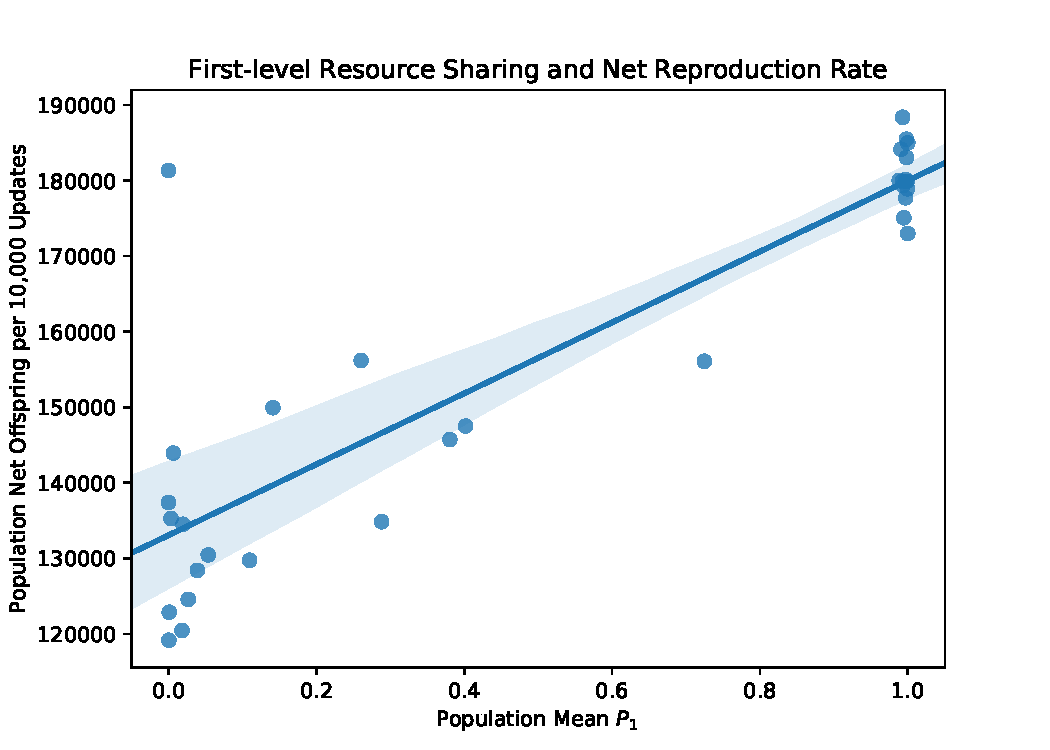
\includegraphics[width=\columnwidth]{img/mean_res_pool2_vs_net_reproduction}
  \caption{
  Correlation plot of population mean $P_2$ and population net reproduction rate.
  }
  \label{fig:mean_res_pool2_vs_net_reproduction}
\end{subfigure}

\caption{
Plot of population mean resource caching strategies and population net reproduction rate.
}
\label{fig:net_reproduction}
\end{center}
\end{figure}


In competition experiments, however, higher-level individuals likely benefited from elimination of somatic mutation.
To assess the relative fitness of first- and second-level individuals without mutation disabled, we examined the relationship between first- and second-level resource pooling and the rate of cellular reproduction at the end of each of the 33 replicate evolutionary trials performed.
We observed a significant negative correlation between mean $P_1$ and cellular reproduction rate ($p < 0.0001$; bootstrap test; Figure \ref{fig:mean_res_pool1_vs_net_reproduction}) and a significant positive correlation between mean $P_2$ and cellular reproduction rate ($p < 0.0001$; bootstrap test; Figure \ref{fig:mean_res_pool2_vs_net_reproduction}).
This result suggests that second-level individuals tend to collect resource more effectively than first-level individuals.
We did not test correlation between $P_{c}$ and reproduction rate due to the small number of trials where cell-level individuality dominated.

\begin{figure}[t]
\begin{center}

\begin{subfigure}[b]{\columnwidth}
  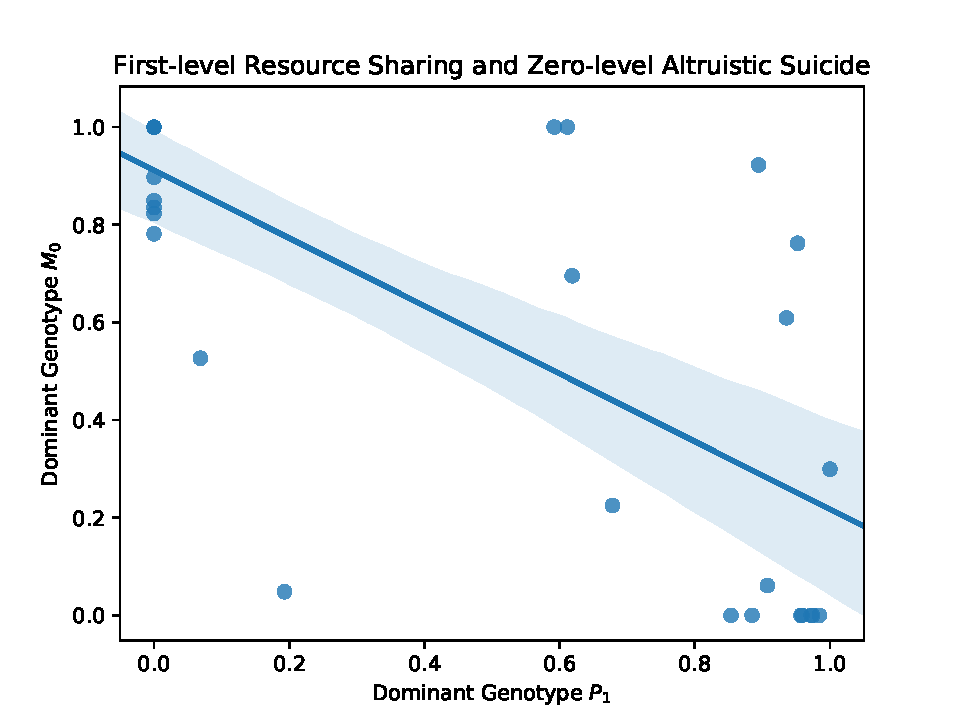
\includegraphics[width=\columnwidth]{img/champion_res_pool1_vs_champion_damage_suicide0}
  \label{fig:champion_res_pool1_vs_champion_damage_suicide0}
\end{subfigure}

\begin{subfigure}[b]{\columnwidth}
  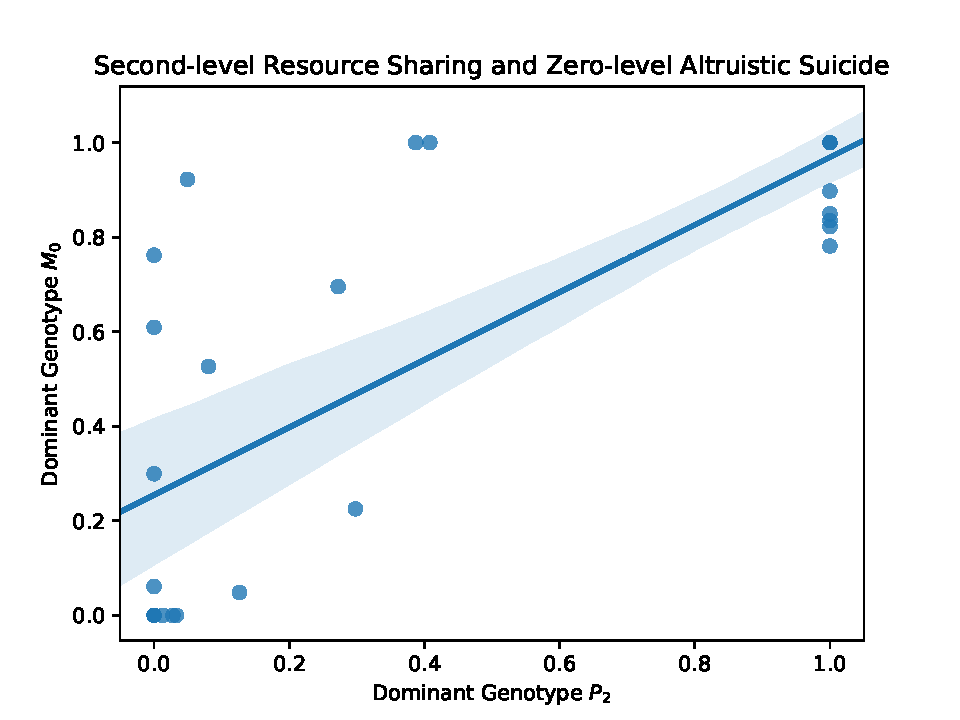
\includegraphics[width=\columnwidth]{img/champion_res_pool2_vs_champion_damage_suicide0}
  \label{fig:champion_res_pool2_vs_champion_damage_suicide0}
\end{subfigure}

\caption{
TODO
}
\label{fig:damage_suicide}
\end{center}
\end{figure}


With the viability of cell-, first-, and second-level individuality in the DISHTINY platform environment --- and the greater relative fitness of second-level individuality --- established, we were also interested in probing the strategies employed by cell-, first-, and second-level individuals beyond resource caching and reproductive deferment.
To assess whether higher-level individuals employed apoptosis to mitigate somatic mutation, we examined the relationship between first- and second-level resource pooling and cellular apoptosis at the conclusion of our 33 replicate evolutionary trials.
We observed a significant negative correlation between dominant genotype $P_1$ and $M_{c}$ ($p < 0.0001$; bootstrap test; Figure \ref{fig:champion_res_pool1_vs_champion_damage_suicide0}) and a significant positive correlation between dominant genotype $P_2$ and $M_{c}$ ($p < 0.0001$; bootstrap test; Figure \ref{fig:champion_res_pool2_vs_champion_damage_suicide0}).
Notably, no genotype encoding second-level individuality was observed with $M_{c} < 0.5$.
This result suggests that second-level individuals, in particular, relied on apoptosis to mitigate somatic mutation, perhaps due to their much larger scale compared to cell- and first-level individuals.

To assess whether higher-level individuals provided larger resource endowments to their propagules (offspring sharing neither the level-one nor the level-two channel ID with the parent), we examined the relationship between first and second-level resource pooling and dominant genotype second-level propagule endowment at the conclusion of our 33 replicate evolutionary trials.
We observed a significant negative correlation between dominant genotype $P_1$ and $E_2$ ($p < 0.001$; bootstrap test) and a significant positive correlation between dominant genotype $P_2$ and $E_2$ ($p <  0.0001$; bootstrap test).
Second-level individuals might provide larger endowments to propagules simply due to a greater capacity to collect resource or perhaps because of stronger selection for well-endowed offspring when competing against other second-level individuals.


\section{Conclusion}

Using simple organisms that evolve parameters for a set of manually-designed strategies, we have demonstrated that DISHTINY environment selects for genotypes that exhibit high-level individuality.
We observed zero-, first-, and second- level individuality among evolutionary outcomes.
Specifically, we observed
\begin{enumerate}
  \item division of reproductive labor between members of the same channel (i.e. between individuals enveloped in a same-channel signaling network and those on the periphery), and
  \item cooperation between members of the same channel (i.e. pooling of resource on the same-channel signaling networks).
\end{enumerate}

Ecological trials revealed that second-level individuals outcompete first- and zero-level individuals.
Interestingly, employment of strategies to combat somatic mutation through apoptosis was correlated with second-level individuality.
We observed that the magnitude of resource endowment for propagules was also correlated with second-level individuality.

Although shifts in individuality coincident with the both the zero- and the one-level signaling network were both clearly observed, the question of whether these transitions were truly hierarchical in nature is debatable.
That is, it is not clear whether first-level individuality was to some extent preserved in or necessary for the emergence of second-level individuality.
Given the nature of the manually-designed strategies for resource-pooling and reproductive division of labor, second-level resource pooling and division of labor could readily leapfrog over first-level resource pooling and division of labor and, in many ways, seemed to completely supersede those first-level efforts.

We believe that this is a shortcoming of the design of organisms employed in these experiments, not the DISHTINY environment itself.
We have nevertheless clearly demonstrated that the DISHTINY environment ultimately selects for high-level individuality.
We are eager to work with more sophisticated cells capable of arbitrary computation via genetic programming in order to pursue more open-ended evolutionary experiments \cite{ofria2004avida}.
Such work will provide valuable insight into scientific questions relating to major evolutionary transitions such as the role of pre-existing phenotypic plasticity \citep{clune2007investigating, lalejini2016evolutionary}, pre-existing environmental interactions, pre-existing reproductive division of labor, and how transitions relate to increases in organizational \citep{goldsby2012task}, structural, and functional \citep{goldsby2014evolutionary} complexity.

We believe that such an approach also provides a unique opportunity to fundamentally further the ambition of the field of Artificial life with respect to open-ended evolution.
Key to this ambition is scale.
The DISHTINY environment near-trivially scales to select for an arbitrary number of hierarchical levels of individuality (not just the two hierarchical levels explored in these experiments).
Importantly, the environment is implemented in a near-completely decentralized manner.
This means that parallelization might be realized --- ultimately, perhaps on the level of the individual toroidal grid tile --- such that per-update run time can nearly remain constant whatever the area of the toroidal grid.
Parallel computing is widely exploited in evolutionary computing, where subpopulations are farmed out to individual compute nodes for for periods of isolated evolution or single genotypes are farmed out to individual compute nodes for fitness evaluation \citep{lin1994coarse, real17a}.
The DISHTINY platform presents a more fundamental parallelization potential: principled parallelization of the evolving individual phenotype at arbitrary scale (i.e. a high-level individual as a large collection of individual cells on the toroidal grid).
Such parallelization will be key to realizing evolving computational systems with scale --- and, perhaps, complexity --- approaching those of biological systems.


\section{Acknowledgements}

Thanks to members of the DEVOLAB, in particular Michael J. Wiser, for feedback on statistical methods.  This research was supported in part by the BEACON Center for the Study of Evolution in Action (NSF Cooperative Agreement No. DBI-0939454) and by Michigan State University through the computational resources provided by the Institute for Cyber-Enabled Research. Any opinions, findings, and conclusions or recommendations expressed in this material are those of the author(s) and do not necessarily reflect the views of the National Science Foundation.


\footnotesize
\bibliographystyle{apalike}
\bibliography{bibl} % replace by the name of your .bib file


\end{document}
